\chapter{Theoretische Grundlagen}

In diesem Kapitel soll einer Kurzer Überblick über die wesentlichen theoretischen Grundlagen gegeben werden, welche später sowohl in der Datenreduktion sowie deren Auswertung Anwendung finden.

\section{Physikalische Grundlagen}

\subsection{Ritchey-Chrétien Teleskop}

Beim Ritchey-Chrétien Teleskop, das eine Weiterentwicklung des Cassegrain-Teleskops darstellt, werden zwei hyperbolisch geformte Spiegel eingesetzt. Dies hat zum Vorteil, dass sphärische Aberrationen und Komafehler eliminiert werden können.

\begin{figure}[htb]
  \centering
  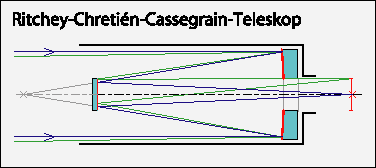
\includegraphics[scale=2]{rc_telescope.pdf}
  \caption[Strahlengang eines Ritchey-Chrétien Teleskops]{Strahlengang eines Ritchey-Chrétien Teleskops mit Fokusebene\cite{rc_telescope}.}
\end{figure}

Analog zum Cassegrain-Teleskop werden die Krümmungsradien der beiden Spiegel wie folgt berechnet:

\begin{align}
	R_1 &= \frac{2DF}{F-B}\\
    R_2 &= \frac{2DB}{F-B-D}
\end{align}
wobei
\begin{itemize}
	\item $F$ die effektive Brennweite des Gesamtsystems,
    \item $B$ der Abstand vom Sekundärspiegel zum Brennpunkt
    \item und $D$ der Abstand der beiden Spiegel ist.
\end{itemize}
Die konischen Konstanten werden dann so gewählt, dass sphärische Aberrationen und Komafehler dritter Ordnung eliminiert werden. Es ergibt sich\cite[S. 508-510]{optical_engineering}

\begin{align}
	K_1 &= -1-\frac{2}{M^3}\cdot\frac{B}{D}\\
    K_2 &= -1-\frac{2}{\left( M-1\right)^3}\left[ M\left( 2M-1\right) +\frac{B}{D}\right]
\end{align}
mit $M=F/f_1=(F-B)/D$ dem sekundären Abbildungsverhältnis. Für das Fraunhofer Teleskop sind diese Kennwerte $K_1=\num{-1.081}$ für den primären und $K_2=\num{-3.601}$ für den sekundären Spiegel\cite{fraunhofer}. Der Primärspiegel ist somit fast parabolisch, wohingegen der Sekundärspiegel hyperbolisch geformt ist. Zusätzlich kommt ein steuerbarer dritter Planspiegel als Fangspiegel zum Einsatz, der das Licht in eine von zwei Nasmyth-Fokusstationen ablenkt.\\
An einem dieser Ports ist eine Weitwinkelkamera (WWFI\cite{wwfi}) montiert, deren Gesichtsfeld etwa \SI{0.5}{\degree} des Himmels abbildet. Da das Bildfeld bei Teleskopen des Typs Ritchey-Chrétien im Allgemeinen nicht eben ist, wird an dem Port des WWFI eine dreilinsige Korrekturoptik eingesetzt, um eine flache Abbildung über \SI{0.7}{\degree} zu ermöglichen. WWFI besitzt ein Mosaik aus $2\times 2$ CCD-Sensoren mit insgesamt 64 Megapixel und ist das Instrument, welche die hier behandelten Fokusreihen aufnimmt.

\subsection{Fokussierung}

Da man es in der beobachtenden Astronomie stets mit praktisch unendlich weit entfernten Objekten zu tun hat, deren Entfernung sich somit auch nicht ändert, wäre es naheliegend, dass nur eine einzige Fokussierung nötig ist um das Teleskop zu eichen um mögliche Fertigungsabweichungen zu berücksichtigen. In der Realität wirken sich Veränderungen der Umgebungsbedingungen wie Verformung durch das Eigengewicht oder Wärmeausdehnung bei Temperaturänderung auf die Optik aus.\\

Für die Verschiebung des Fokus durch die Temperatur lässt sich folgende Überlegung anstellen. Der Längenausdehnungskoeffizient $\alpha$ eines Festkörpers der Länge $L$ ist definiert als die relative Längenänderung pro Temperaturänderung $\Delta T$.
\begin{align}
	\alpha &= \frac{\Delta L}{L\cdot \Delta T}
\end{align}
Für die temperaturabhängige Länge ergibt sich nach Integration
\begin{align}
	L(T) &= L(T_0)\cdot \exp[\int_{T_0}^T\alpha(T)\dd{t}].
\end{align}
Mit der Annahme, dass der Koeffizient nicht von der Temperatur abhängt, also $\alpha(T) = \alpha(T_0)$, lässt sich die Differentialgleichung gleich lösen.
\begin{align}
	L(T) &= \underbrace{L(T_0)}_{\equiv L_0}\cdot \exp[\alpha\cdot (\underbrace{T-T_0}_{\equiv \Delta T})]
\end{align}
Oder als Taylorentwicklung bis zur Ordnung $\mathcal{O}(\Delta T)$:
\begin{align}
	L &\approx L_0(1+\alpha\cdot\Delta T)\\
    \Rightarrow \Delta L &\approx \alpha \cdot L_0\cdot \Delta T
\end{align}
Die Fokusverschiebung durch die Temperaturänderung ist also für kleine $\Delta T$ in guter Näherung linear. Auf ähnliche Weise lässt sich argumentieren, dass die Verformung des Teleskops, die ja winkelabhängig von der Neigung des Teleskops ist, in erster Näherung zu einer linearen Stauchung und somit auch zu einer linearen Fokusverschiebung führt. Entsprechendes konnte für das Fraunhofer Teleskop in der Vergangenheit schon nachgewiesen werden\cite{commissioning}. Aufgrund der komplexen Geometrie des Teleskops und der verschiedenen Materialien ist es allerdings naheliegend, dass die wahre Funktion der Fokusverschiebung komplizierter ist.

\subsection{Aberrationen}

Die Zernike-Polynome bilden eine orthogonale Basis die verwendet werden kann um eine Wellenfront zu repräsentieren. Somit können Zernike-Polynome auch die Abbildungsfehler eines optischen Systems beschreiben.\\
Die Fokusserien, welche in dieser Arbeit behandelt werden, wurden bereits auf die Koeffizienten relevanter Zernike-Polynome reduziert. Dazu wurden für die Sterne in jeder Aufnahme mit der Donut Methode, wie beschrieben von Tokovinin und Heathcode 2006\cite{donut}, die Momente zweiter Ordnung berechnet.

\begin{mdframed}[style=emphasis]
\emph{Momente} in der Bildverarbeitung werden aus den gewichteten Mittelwerten der normierten Helligkeitswerte einzelner Pixel gebildet. Sie können dabei so gewählt werden, dass sie bestimmte Eigenschaften eines Bildes widerspiegeln oder gewisse geometrische Interpretationen besitzen. Insbesondere sind Momente hilfreich, um einzelne Objekte in einem segmentierten Bild zu beschreiben.
\end{mdframed}
Mit Hilfe der Momente werden folgende Koeffizienten definiert, die direkt proportional zu den entsprechenden Zernike Koeffizienten mit Noll-Indizes\cite{noll} sind.
\begin{align}
	A_4 &= p\sqrt{(M_x + M_y)/2}\\
    A_5 &= pM_{xy}(M_xM_y)^{-1/4}\\
    A_6 &= 0.5p(M_x-M_y)(M_xM_y)^{-1/4}
\end{align}
Dabei ist $p$ die Winkelausdehnung der Detektor Pixel. Diese Koeffizieten werden als Maß für Defokus ($A_4$) sowie schrägen und senkrechten Astigmatismus ($A_5, A_6$ resp.) verwendet.
\section{Statistische Grundlagen}
\subsection{B-Spline Interpolation}
Ein B-Spline der Ordnung $k$ wird gebildet, in dem man mehrere Polynome des Grads $k-1$, die maximal $C^{k-2}$ stetig an den Endpunkten sind, aneinanderhängt. Dabei definiert der aufsteigende Satz der Endpunkte $t_0 \le t_1 \le \ldots \le t_m$ den sog. Knotenvektor
\begin{align*}
	\va{T} = (t_0,t_1,\ldots,t_m),
\end{align*}
der die Parametrisierung der Basisfunktionen festlegt. Die Definition der Basisfunktionen, die sich als besonders numerisches stabil herausgestellt hat, ist wie folgt\cite{b-splines}:
\begin{align}
	N_{i,1}(t) &= \begin{cases}1 \text{ für } t_i \le t \le t_{i+1}\\0\text{ sonst}\end{cases}\\
    N_{i,k}(t) &= \frac{t-t_i}{t_{i+k-1}-t_i}N_{i,k-1}(t)+\frac{t_{i+k}-t}{t_{i+k}-t_{i+1}}N_{i+1,k-1}(t)\label{bspline}
\end{align}
für $i=0,1,\ldots,n$. Gleichung \eqref{bspline} gilt dabei für $k > 1$.\\
Eine B-Spline Kurve lässt sich dann schreiben als eine Linearkombination von Kontrollpunkten $\vb{p}_i$ und Basisfunktionen:
\begin{align}
	r(t) &= \sum_{i=0}^n\vb{p}_i N_{i,k}(t),\qquad n\ge k-1,\qquad t\in [t_{k-1},t_{n+1}].
\end{align}
Eine Parametrisierung der Form $f(x, y)=z$ lässt sich nun mit Hilfe einer B-Spline Fläche interpolieren. Die B-Spline Fläche ist das Tensorprodukt zweier B-Splines und wird daher definiert durch einen rechteckigen Satz an Kontrollpunkten $\vb{p}_{ij},0\le i\le m, 0\le j \le n$ und zwei Knotenvektoren $\va{X} = (x_0,x_1,\ldots,x_{m+k})$ und $\va{Y} = (y_0,y_1,\ldots,y_{n+l})$ entsprechend der veränderlichen $x$ und $y$.
Die Fläche ist dann gegeben durch
\begin{align}
	f^*(x, y) = \sum_{i=0}^m\sum_{j=0}^n \vb{p}_{ij} N_{i,k}(x)N_{j,l}(y).
\end{align}
Die nötigen Kontrollpunkte können mit einem QuickHull Algorithmus bestimmt werden\cite{surface}. Insbesondere sind die Kontrollpunkte im Gegensatz zu Bézierkurven nicht notwendigerweise Teil des Interpolanten. Durch Wiederholen eines Punktes im Knotenvektor kann die Differenzierbarkeit des Interpolanten an diesem Punkt um jeweils $1$ heruntergesetzt werden. Ein Knotenpunkt der Multiplizität $k$ für ein B-Spline $k$-ter Ordnung zwingt den Interpolanten somit den Wert des Knotenpunkts an der entsprechenden Stelle anzunehmen.\\
Eine so bestimmte Interpolations-Fläche nimmt zwar an den Eckpunkten garantiert die Werte der Knotenvektoren ein, ist allerdings auch nur innerhalb der von den Knotenvektoren aufgespannten konvexen Hülle definiert. Möchte man, dass dieser Interpolant auch Werte für Regionen außerhalb seiner konvexen Hülle liefert, müssen diese extrapoliert werden.
\subsection{Korrelation und Transinformation}
Die Korrelation beschreibt den statistischen Zusammenhang zweier Ereignisse. Dieser Zusammenhang muss dabei nicht notwendigerweise auf eine kausale Beziehung zurückzuführen sein und kann rein stochastischer Natur sein.\\
Im Rahmen dieser Arbeit wird die Korrelation diskreter Wahrscheinlichkeitsverteilungen untersucht. Das Mittel der Wahl stellt die Transinformation (auch engl. \emph{mutual information}) dar. Sie ist ein Maß für die Korrelation der Distributionen, welche im Vergleich zum Korrelationskoeffizienten nicht nur lineare sondern auch nicht-lineare Abhängigkeiten berücksichtigt\cite{mi_corr}.\\
Die Transinformation kann auch als Wert interpretiert werden, der angibt wie sehr die multivariate Verteilung $p(X, Y)$ dem Produkt der Verteilungen $p(X) p(Y)$ ähnelt. Formal kann sie dann definiert werden als:
\begin{align}
	I(X,Y) &= \sum_{y\in Y}\sum_{x\in X}p(x,y)\log(\frac{p(x,y)}{p(x)p(y)})
\end{align}
mit der multivariaten Wahrscheinlichkeitsdichtefunktion $p(x, y)$ der Mengen $X$ und $Y$ sowie $p(x)$ und $p(y)$ den Randverteilungen von $X$ und $Y$ respektive. Handelt es sich um unabhängige Verteilungen, so faktorisiert $p(x, y)$ und der Transinformationsgehalt ist folglich $\num{0}$, da für den Logarithmus gilt:
\begin{align}
	\log(\frac{p(x)p(y)}{p(x)p(y)}) = \log(1) = 0.
\end{align}
Im weiteren kann die Transinformation noch normiert werden, wenn man sie als Kovarianz und die Shannon-Entropie analog als Varianz interpretiert\cite{mi_norm}:
\begin{align}
	I_{\mathrm{norm}}(X,Y) &= \frac{I(X,Y)}{\sqrt{H(X)H(Y)}}
\end{align}
mit $H(X)$ und $H(Y)$ der Shannon-Entropie der jeweiligen Verteilungsfunktion.